\section{計算領域(格子数・解像度・MPIプロセス数)の指定}
\label{sec:domain}
%=======================================================================

水平格子間隔と格子数が計算領域を決定するのは言うまでもないが、
SCALEではMPIプロセス数も考慮する必要がある。
図X%\ref{fig:domain}
は、計算領域、及び、水平格子間隔、格子数、MPIプロセス数の関係を示している。


%\begin{figure}[h]
%\begin{center}
%  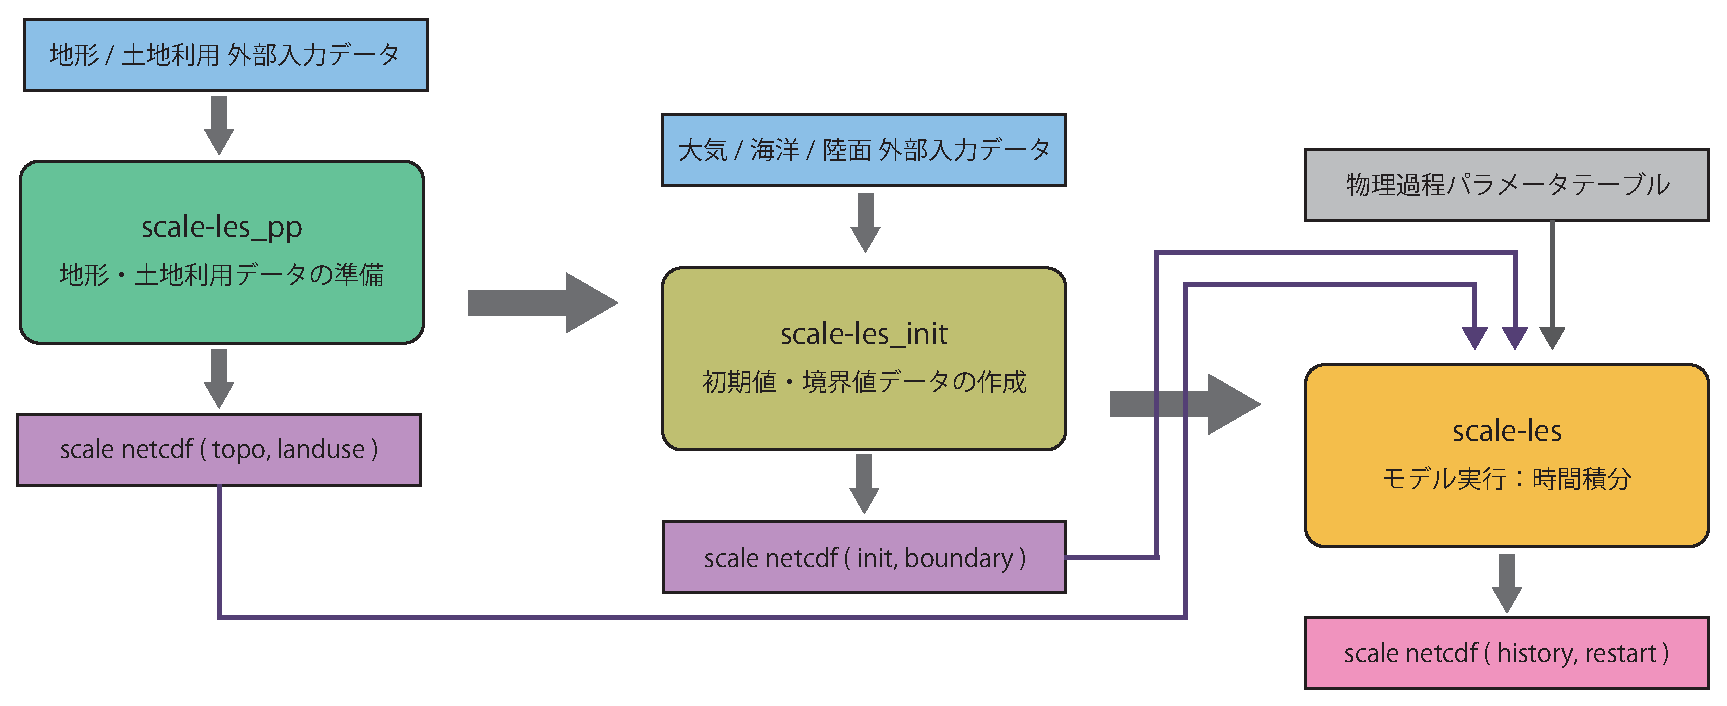
\includegraphics[width=0.9\hsize]{./figure/how_to_run.eps}\\
%  \caption{SCALE-RMモデルの実行過程}
%  \label{fig:howto}
%\end{center}
%\end{figure}


計算領域は、MPIプロセス数(n=\verb|PRC_NUM_X|$\times$\verb|PRC_NUM_Y|)が
2以上の時は、計算領域を水平方向にn個に分割して行う。
namelistで設定する格子数(\verb|IMAX|, \verb|JMAX|, \verb|KMAX|)は、
1つのMPIプロセスが担当する格子点数を与える仕様となっている。
以上の関係から、計算領域の全体の総格子点数は下記のように計算される。

\begin{eqnarray}
 総格子数 = (\verb|IMAX| \times \verb|PRC_NUM_X|)
   \times (\verb|JMAX| \times \verb|PRC_NUM_Y|)
   \times (\verb|KMAX| )  \nonumber
\end{eqnarray}


次節以降では、格子間隔、格子数、MPIプロセス数それぞれの設定方法について詳しく説明する。


\subsection{水平・鉛直格子間隔}
%-----------------------------------------------------------------------
SCALEでは、格子点の位置を均等間隔に設定することも、
任意の格子点位置を直接指定することもできる。
以下で説明する
\textcolor{red}{\bf 格子間隔の設定は、pp\_***.conf、init\_***.conf、run\_***.confの
configファイルの間で一致させなければならないことに注意が必要である。}
また、以下で設定する値は、MPIプロセス当たりの値であることに注意が必要である。


\subsubsection{均等間隔で設定する場合}
%-----------------------------------------------------------------------&
configファイルの\verb|PARAM_GRID|の\verb|DX|、\verb|DY|、\verb|DZ|に
それぞれ、東西、南北、鉛直方向の格子間隔を指定する。

\noindent {\small {\gt
\ovalbox{
\begin{tabularx}{140mm}{lX}
\verb|&PARAM_GRID  | & \\
\verb| DX = 500.D0,| & ; X方向(東西方向)の格子間隔\\
\verb| DY = 500.D0,| & ; Y方向(南北方向)の格子間隔\\
\verb| DZ = 500.D0,| & ; Z方向(鉛直方向)の格子間隔\\
\verb|/|\\
\end{tabularx}
}}}\\


\subsubsection{任意の格子点位置を指定}
%-----------------------------------------------------------------------&
SCALEの格子系はArakawa-Cグリッド、
およびLorenzグリッドであるため、水平方向と鉛直方向ともに
スタッガード点(1/2ずれた点)に変数が定義されている。
コントロールボリュームに対して中心点に位置する格子点を
Center Pointと呼び、コントロールボリュームの面に位置する格子点
(Center Pointに対して1/2ずれている)をFace Pointと呼ぶ。
SCALEでは、これらの頭文字と方向を組み合わせて
\verb|CX、CY、CZ|や\verb|FX、FY、FZ|と呼ぶ
(図\ref{fig:scale_grid})。

\begin{figure}[h]
\begin{center}
  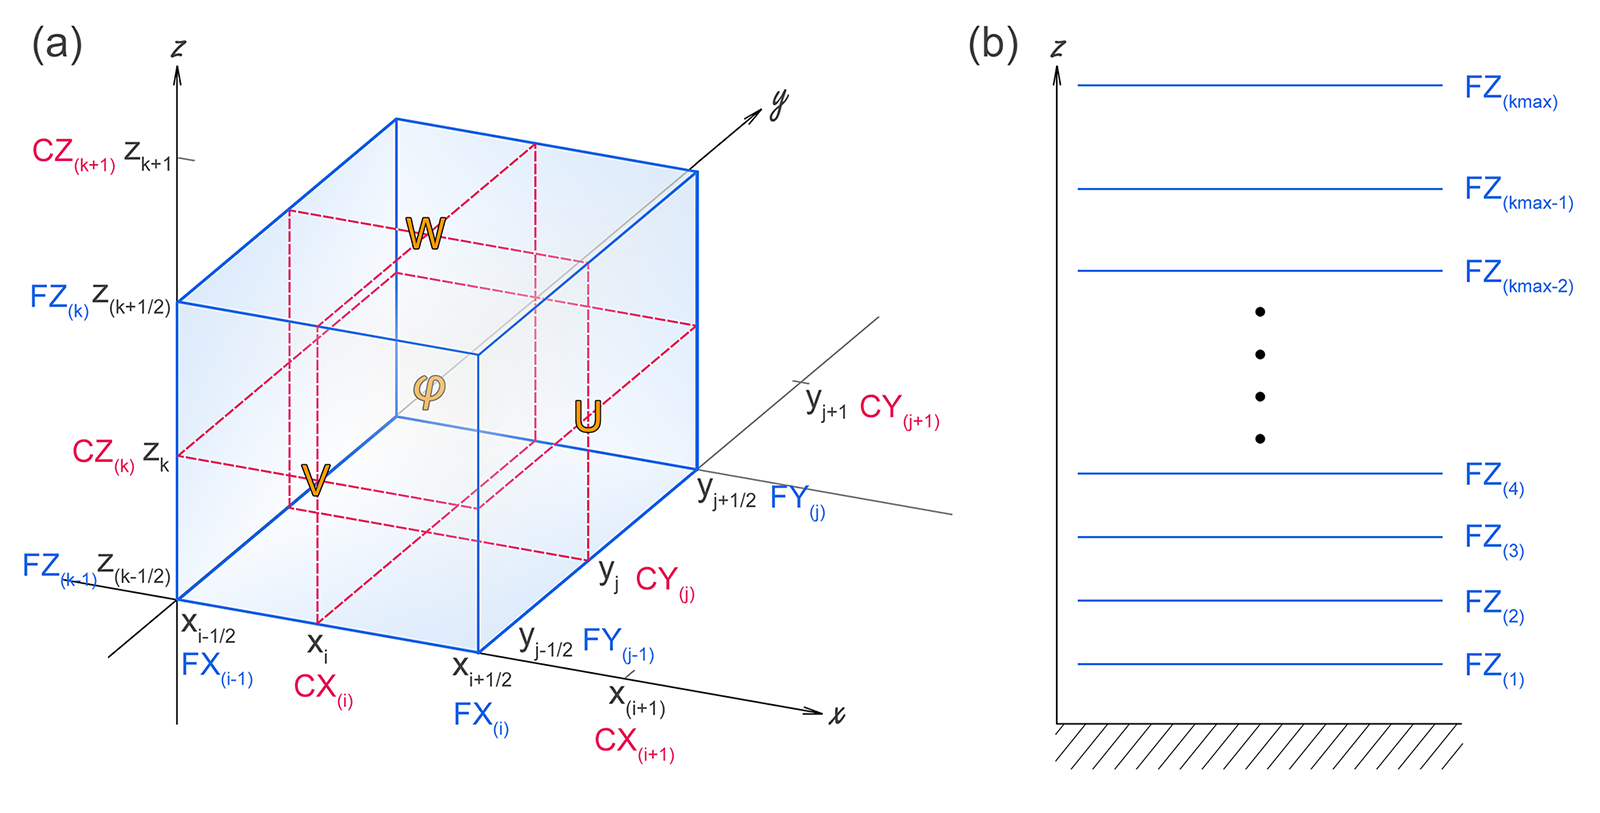
\includegraphics[width=0.8\hsize]{./figure/Center-Face.eps}\\
  \caption{SCALE-RMの格子の定義}
  \label{fig:scale_grid}
\end{center}
\end{figure}


直接格子点の位置を指定する場合は、
Center PointもしくはFace Pointの位置を明記すれば良い。
これらの変数の単位はメートル[m]である
\footnote{指定の際には、シミュレーションの計算精度(モデルのコンパイル時に指定した浮動小数点の精度。
デフォルトでは倍精度)を用いることが望ましい。}

例として理想実験のチュートリアルのrun.confファイル
(run\_R20kmDX500m.conf)を下記に示す。\\

\noindent {\small {\gt
\ovalbox{
\begin{tabularx}{140mm}{l}
\verb|&PARAM_GRID|\\
\verb| DX = 500.D0,|\\
\verb| DY = 500.D0,|\\
\verb| FZ(:) = |\\
\verb|    80.000000000000000      ,|\\
\verb|    168.00000190734863      ,|\\
\verb|    264.80000610351567      ,|\\
\verb|     〜 中略 〜|\\
\verb|    14910.428862936289      ,|\\
\verb|    15517.262523292475      ,|\\
\verb|    16215.121232702089      ,|\\
\verb|    17017.658748523147      ,|\\
\verb|    17940.576891717363      ,|\\
\verb|    19001.932756390710      ,|\\
\verb|    20222.492000765058      ,|\\
\verb| BUFFER_DZ = 5000.D0,|\\
\verb| BUFFFACT  =   1.0D0,|\\
\verb|/|\\
\end{tabularx}
}}}\\

%\verb|DX|、\verb|DY|は``\verb|500.D0|''と倍精度表記を用いて500 mと指定されており、
%水平方向の格子間隔は500 mの均等間隔に設定されていることがわかる。
%一方、
\verb|FZ(:)|は、鉛直方向のFace pointの位置を直接指定している。
\verb|FZ(:)|で指定する値の数は、
鉛直層数(\verb|PARAM_INDEX|の\verb|KMAX|、次節で説明)
と一致させる必要がある。
%
格子点位置を任意に設定できるといっても、設定が悪いと計算不安定につながる。
鉛直層設定の作成をサポートするツールを
\verb|scale/scale-rm/util/makevgrid|
\footnote{``make\_vgrid.f90''というFortranプログラムと
いくつかのサンプルnamelistが用意されている。
これをコンパイルして実行すれば直ちにconfigファイルに貼り付けて使用できる
フォーマットの鉛直層設定を作成できる。}
に用意しているので、それを使って生成することを勧める。


\subsection{水平・鉛直格子数}
%-----------------------------------------------------------------------

格子数の設定は、configureファイルの\verb|PARAM_INDEX|で行う。
以下で設定する水平格子数の値は、
MPIプロセス当たりの値であることに注意が必要である。\\

\noindent {\small {\gt
\ovalbox{
\begin{tabularx}{140mm}{lX}
\verb|&PARAM_INDEX| & \\
\verb| KMAX = 97,|  & 鉛直層数 \\
\verb| IMAX = 20,|  & X方向の格子点数 \\
\verb| JMAX = 2, |  & Y方向の格子点数 \\
\verb|/|\\
\end{tabularx}
}}}\\



%さて、上記の設定を変更して4-MPI並列で実行できるようにしてみる。注意する点は領域全体の格子点数を
%維持するように設定することである。今回は準2次元実験なので、X方向に4分割して4-MPI並列を達成する。
%この場合の設定方法は下記のとおりである。\\

%\noindent {\small {\gt
%\ovalbox{
%\begin{tabularx}{140mm}{l}
%\verb|&PARAM_INDEX|\\
%\verb| KMAX = 97,|\\
%\verb| IMAX = 10,|\\
%\verb| JMAX = 2,|\\
%\verb|/|\\
%\\
%\verb|&PARAM_PRC|\\
%\verb| PRC_NUM_X       = 4,|\\
%\verb| PRC_NUM_Y       = 1,|\\
%\verb|/|\\
%\end{tabularx}
%}}}\\

%\noindent X方向に4分割を指定するため、\verb|PRC_NUM_X = 4|と記述されている。そして、領域全体で40格子点
%とするために、\verb|IMAX = 10|と記述されている。Y方向と鉛直方向には何も変更していない。
%\textcolor{red}{この変更を、{\bf init\_R20kmDX500m.conf}と{\bf run\_R20kmDX500m.conf}の両方に施さなければならない。}
%そして、つぎのようにMPIコマンドに指定するプロセス数を``4''として、初期値作成、モデル実行の順で
%作業を進めれば、4-MPI並列で実行することができる。
%\begin{verbatim}
%  $ mpirun  -n  4  ./scale-rm_init  init_R20kmDX500m.conf
%  $ mpirun  -n  4  ./scale-rm       run_R20kmDX500m.conf
%\end{verbatim}

%計算領域(総演算量)を維持したままMPIプロセス数を
%2倍に増やすことによって、プロセス数に応じて使用するコア数も
%2倍となる場合、1つのMPIプロセスあたりの
%問題サイズ(演算量 per PRC)が1/2に減る。
%したがって、計算にかかる時間も理想的には半分になる
%%\footnote{計算科学用語では、この変更、つまり総演算量一定でプロセスあたりの演算量を減らしていくことを``strong scaling''と呼ぶ。}。
%実験機では、2-MPI並列のときチュートリアルの時間積分に60 sec かかっていたが、4-MPI並列にすることで同じ計算が32 secで終了できた。
%ここで説明したMPIプロセス数の変更を加えたサンプルファイルが、同じディレクトリ下の``sample''ディレクトリ内に
%\verb|init_R20kmDX500m.pe4.conf|、\verb|run_R20kmDX500m.pe4.conf|として置いてあるので、うまく実行できない場合は
%参考にして欲しい。



\subsection{MPIプロセス数}

MPIプロセス数は、各confファイルの\verb|PARAM_PRC|で指定する。
先に述べた通り、SCALEの入出力ファイルは、MPIプロセス毎に分割されている。
そのため、MPIプロセス数を変更すると分割ファイル数も必ず変わることになる。
従って、例えば、2-MPI並列用に作成した初期値ファイルは、
4-MPI並列のモデル実行には使用できない。
MPIプロセス数を変更するには、
\verb|pp_***.conf|、\verb|init_***.conf|、\verb|run_***.conf| の
すべてを編集・変更し、\verb|pp|, \verb|init| から行わなければならない。\\

\noindent {\small {\gt
\ovalbox{
\begin{tabularx}{140mm}{lX}
\verb|&PARAM_PRC| & \\
\verb| PRC_NUM_X       = 2,| & X方向(東西方向)のMPI並列分割数 \\
\verb| PRC_NUM_Y       = 1,| & Y方向(南北方向)のMPI並列分割数 \\
\verb|/|\\
\end{tabularx}
}}}\\


全MPIプロセス数は、\verb|PRC_NUM_X| $\times$ \verb|PRC_NUM_Y|  となり、
上記の例では、X方向に2分割、Y方向に1分割(分割なし)の
2-MPI並列ということになる。

実行時にMPIコマンドに指定するMPIプロセス数は、
この総MPIプロセス数を指定しなければならない。
この条件を満たさない場合は,LOGファイルなどに\\

\noindent {\small {\gt
\ovalbox{
\begin{tabularx}{140mm}{l}
\verb|xxx total number of node does not match that requested. Check!| \\
\end{tabularx}
}}}\\

\noindent というメッセージが出力がされて計算が異常終了する。




\subsection{計算領域の変更の練習問題}
ここでは、現実大気実験のチュートリアルのconfigファイル(\verb|run.conf|)を元にしていくつかの変更例を説明する。
以下の変更例をもとに、自分の行いたい実験設定にあったconfigファイルを作り上げてもらいたい。\\


{\bf a. MPIプロセス数はそのままに計算領域を4倍に広げる}\\

この設定はとても簡単である。デフォルト設定は、X方向、Y方向ともに2つのMPIプロセスを使用し、格子点数はともに
30点なので、全領域の格子点数は、$(2 \times 60)_{x} \times (2 \times 60)_{y} = 14400$点である。
従って、計算領域を4倍に広げるためには、\verb|IMAX|、\verb|JMAX|の値をデフォルトに対して2倍の値に変更するだけである。
これで、全領域の格子点数は、$(2 \times 120)_{x} \times (2 \times 120)_{y} = 57600$点となり、14400点の4倍の
計算領域になっている。この変更を施したconfigファイルの例は次のとおりである。
赤文字の部分がデフォルトからの変更点を意味する。\\

\noindent {\small {\gt
\ovalbox{
\begin{tabularx}{140mm}{l}
\verb|&PARAM_PRC| \\
\verb| PRC_NUM_X      = 2,| \\
\verb| PRC_NUM_Y      = 2,| \\
\verb| PRC_PERIODIC_X = .false.,| \\
\verb| PRC_PERIODIC_Y = .false.,| \\
\verb|/| \\
 \\
\verb|&PARAM_INDEX| \\
\verb| KMAX = 36,| \\
\textcolor{red}{\verb| IMAX = 120,|} \\
\textcolor{red}{\verb| JMAX = 120,|} \\
\verb|/| \\
\end{tabularx}
}}}\\

\vspace{5mm}
{\bf b. 1つのMPIプロセスあたりの格子点数はそのままに計算領域を4倍に広げる}\\

先程は、MPIプロセス数を維持して計算領域を広げたが今度は、1つのMPIプロセスあたりの格子点数はそのままに、MPIプロセス数を
増やすことで計算領域を4倍に広げる方法を説明する。1つのMPIプロセスあたりの格子点数(プロセスあたりの演算量)は
そのままにMPIプロセス数を増やすことで計算領域を広げる(総演算量を増やす)。この場合、1つのCPUが担当する問題サイズは
変わらないため、理想的には計算にかかる時間を増やすことなく計算領域を広げることができる
\footnote{計算科学用語では、この変更、つまりプロセスあたりの演算量一定で総演算量を増やしていくことを``weak scaling''と呼ぶ。}。

計算領域を4倍に広げるためには、\verb|PRC_NUM_X|、\verb|PRC_NUM_Y|の値をデフォルトに対して2倍の値に変更するだけである。
これで、全領域の格子点数は、$(4 \times 60)_{x} \times (4 \times 60)_{y} = 57600$点となり、14400点の4倍の
計算領域になっている。このとき必要なMPIプロセス数は、$4 \times 4 = 16$プロセス、つまりデフォルトの4倍のMPIプロセス数が必要になる。
この変更を施したconfigファイルの例は次のとおりである。赤文字の部分がデフォルトからの変更点を意味する。\\

\noindent {\small {\gt
\ovalbox{
\begin{tabularx}{140mm}{l}
\verb|&PARAM_PRC| \\
\textcolor{red}{\verb| PRC_NUM_X      = 4,|} \\
\textcolor{red}{\verb| PRC_NUM_Y      = 4,|} \\
\verb| PRC_PERIODIC_X = .false.,| \\
\verb| PRC_PERIODIC_Y = .false.,| \\
\verb|/| \\
 \\
\verb|&PARAM_INDEX| \\
\verb| KMAX = 36,| \\
\verb| IMAX = 60,| \\
\verb| JMAX = 60,| \\
\verb|/| \\
\end{tabularx}
}}}\\

\vspace{5mm}
{\bf c. 計算領域はそのままに水平格子間隔を3 kmに変更する}\\

現実大気実験チュートリアルのデフォルト設定は、X方向、Y方向の総格子点数は120点で水平格子間隔が15 kmなので、
計算領域は1800 km $\times$ 1800 kmの領域となっている。ここでは、この領域を維持したまま水平格子間隔を3 kmに
狭める設定にトライする。水平格子間隔が15 kmから3 kmへ1/5だけ小さくなるので逆に1方向あたりの総格子点数は5倍、
つまり600点必要になる。この600点をどのようにMPIプロセス数とプロセスあたりの格子点数として割り振るかは
ユーザーの環境や計算機リソース量によって異なる。たとえば、X方向、Y方向ともに10プロセスずつ、合計で100プロセスを
使えば、プロセスあたりの格子点数は60点となり、積分時間間隔が短くなることを無視すれば演算量はデフォルトと変わらない。

しかし、なかなか100プロセスを利用できる計算機を持っている環境にいる人は少ないだろう。そこで、デフォルトから
各方向に1つずつMPIプロセス数を増やし、$3 \times 3 = 9$プロセスを利用した設定を考えてみる。
1方向あたりの総格子点数は600点なので、プロセスあたりの格子点数は$600 \div 3 = 200$点となる。

ここでの変更で気をつけなければならないことは、バッファー領域の幅である。現実大気実験チュートリアルの
デフォルト設定ではバッファー領域は、計算領域トップと東西南北の側面境界に設定されており、側面境界のバッファー領域の
幅は片側300 km、つまり15 km格子間隔で20点のバッファー格子点が確保されている。水平格子間隔を15 kmから3 kmへ変更
したので、このままでは100点もの格子点がバッファー領域に取られてしまう。SCALEでは一般的に20〜40点程度の
バッファー格子点を設定するようにしているので、デフォルトと同じ20点になるように側面境界のバッファー領域の
幅は片側60 kmと設定する。鉛直層設定は変更していないため、計算領域トップのバッファー領域については設定を変更する
必要はない。

この変更を施したconfigファイルの例は次のとおりである。赤文字の部分がデフォルトからの変更点を意味する。\\

\noindent {\small {\gt
\ovalbox{
\begin{tabularx}{140mm}{l}
\verb|&PARAM_PRC| \\
\textcolor{red}{\verb| PRC_NUM_X      = 3,|} \\
\textcolor{red}{\verb| PRC_NUM_Y      = 3,|} \\
\verb| PRC_PERIODIC_X = .false.,| \\
\verb| PRC_PERIODIC_Y = .false.,| \\
\verb|/| \\
 \\
\verb|&PARAM_INDEX| \\
\verb| KMAX = 36,| \\
\textcolor{red}{\verb| IMAX = 200,|} \\
\textcolor{red}{\verb| JMAX = 200,|} \\
\verb|/| \\
 \\
\verb|&PARAM_GRID| \\
\textcolor{red}{\verb| DX = 3000.D0,|} \\
\textcolor{red}{\verb| DY = 3000.D0,|} \\
\verb| FZ(:) =    80.841D0,   248.821D0, ... ... 1062.158D0,| \\
\verb|            1306.565D0,  1570.008D0, ... ... 2845.575D0,| \\
\verb|       〜 中略 〜|\\
\verb|           18387.010D0, 19980.750D0, ... ... 28113.205D0,| \\
\verb| BUFFER_DZ = 5000.D0,| \\
\textcolor{red}{\verb| BUFFER_DX = 60000.D0,   ! 20 buffer|} \\
\textcolor{red}{\verb| BUFFER_DY = 60000.D0,   ! 20 buffer|} \\
\verb|/| \\
\end{tabularx}
}}}\\

